\documentclass{article}
\usepackage{circuitikz}
\usepackage{siunitx}
\begin{document}
\begin{figure}[h]
    \centering
    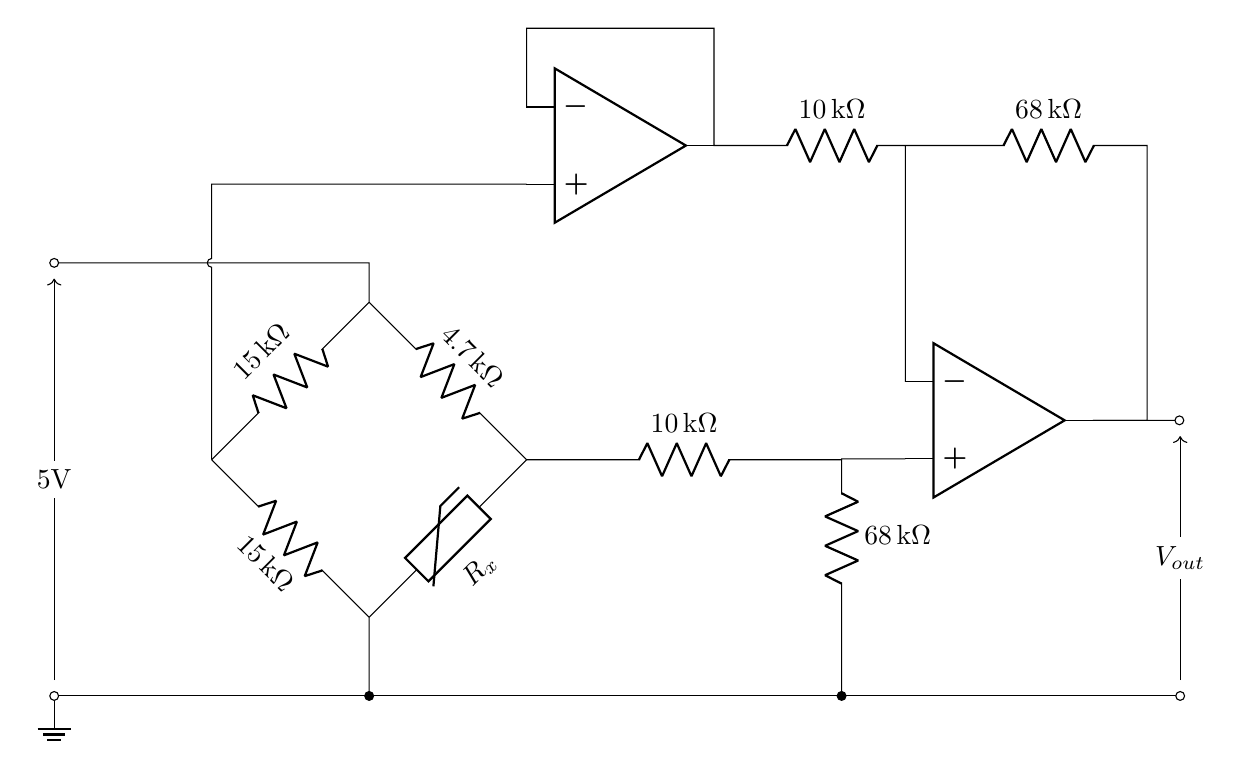
\begin{tikzpicture}
        \draw (-1,-2) node[ground]{} to[short, o-o] (13.3,-2); %Ground
        \draw [->] (-1,-1.8) -- node[fill=white]{5V}(-1,3.3); %V_in
        \draw [->] (13.3,-1.8) -- node[fill=white]{$V_{out}$} (13.3,1.3); %V_out
        \draw
            (-1,3.5) to[short,o-] (0,3.5) |- (3,3.5) to[short] ++ (0,-0.5)
            (3,3) to [R,a=$\SI{15}{k\ohm}$] (1,1) %Top left resistor
            (3,3) to [R,l=$\SI{4.7}{k\ohm}$] (5,1) %Top right resistor
            (1,1) to [R,a=$\SI{15}{k\ohm}$] (3,-1) %Bottom right resitor
            (5,1) to [thermistor,l=$R_x$] (3,-1) %Bottom left resistor
            (3,-1) to[short, -*] ++  (0,-1) %Connection to ground
        ;
        \node [op amp] (opamp) at (11,1.5) {}; %Create Op amp 
        \draw
            (opamp.out) to[short,-o] ++ (1.1,0) %Draw output to V_out
            (5,1) to[R,l=$\SI{10}{k\ohm}$] ++(4,0) coordinate (x) |- (opamp.+)
            (x) to[R, l=$\SI{68}{k\ohm}$] ++(0,-2) to[short,-*] ++ (0,-1)
        ;
        \draw
            (1,1) -- ++ (0,2) to[crossing] ++ (0,1) %From left-bridge towards buffer
            |- ++ (4,0.5) node[op amp, anchor=+] (buffer) {} %Create buffer
            (buffer.-) -- ++ (0,1) -| (buffer.out) %connect inverting input and output
            to [R,l=$\SI{10}{k\ohm}$] ++ (3,0) coordinate (y)
            -| (opamp.-) %Betwen 10k and 68k to inverting input
            (y) to[R,l=$\SI{68}{k\ohm}$] ++ (2.5,0)
            |- (opamp.out) %68k to output  
        ;
    \end{tikzpicture}
\end{figure}
\end{document}